\newpage
\chapter{Background}

\section{Information Retrieval}

The following definition of Information Retrieval (IR) was given by \textit{Gerard Salton} in 1968 and is still accurate nowadays \cite{croftIR}:

\begin{quote}
``Information retrieval is a field concerned with the structure, analysis, organization, storage, searching, and retrieval of information''.
\end{quote}

This definition is very general, in fact IR refers to a wide range of applications related to search.

The primary focus of the field since the 1950s has been on textual data (e.g. web pages, email, scholarly papers, books, and news). This type of data is mostly unstructured, thus matching between two pieces of text is not that easy: understanding and modeling how people compare texts, and designing algorithms to accurately perform this matching, is at the core of IR.

One typical \textbf{task} involves a user submitting a query to a \textbf{search engine} (a practical application of IR techniques to large-scale text collections) and receiving a list of documents in \textbf{ranked order}.

Such order depends on \textbf{relevance}, a key and complex concept in IR. Although there is not a formal definition, it can be described as the likelihood of an information to satisfy the user need.

There are many factors that influence whether a user considers relevant or not a document (e.g. contextual factors, time, location, language \dots).

Sometimes a document which is \textbf{topical relevant} to a query (i.e. that talks about the same topic) may not be \textbf{relevant to the user} (i.e. that satisfy the user information need).

To address the issue of relevance, researchers propose various retrieval models and test how well they work through experimental evaluation (later described).

A \textbf{retrieval model} is a formal representation of the process of matching a query and a document. It is part of the ranking algorithm that is used in a search engine to produce the ranked list of documents.

A good retrieval model will find documents that are likely to be considered relevant by the person who submitted the query.

\section{Principal components of a retrieval systems}
\label{sec:rspc}

Search engine components support two major functions: the indexing process and the query process \cite{croftIR}.

The indexing process builds the structures that enable searching and the query process uses those structures and a query submitted by a user to produce a ranked list of documents. 

\subsection{Indexing}

The major components of indexing are text acquisition, text transformation, and index creation (picture \ref{fig:indexing}).

\begin{figure}
  \centering
  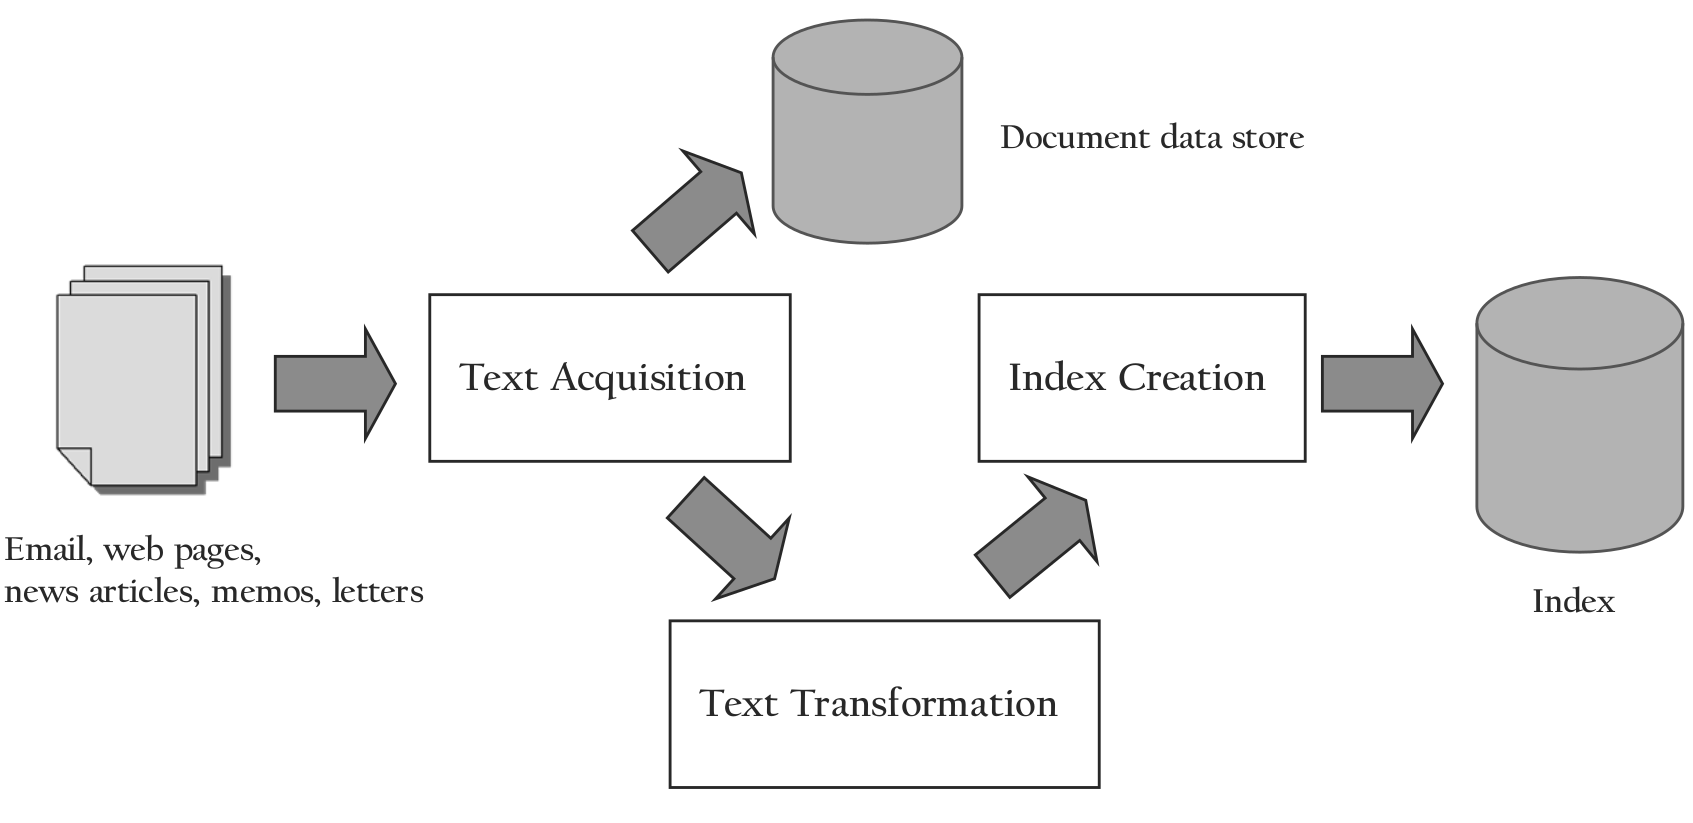
\includegraphics[width=0.9\textwidth]{indexing.png}
  \caption{The indexing process (picture taken from \cite{croftIR})}
  \label{fig:indexing}
\end{figure}

\textbf{Text acquisition} is the process of acquiring the documents that will be searched.

Although in some cases this will involve simply using an existing collection, text acquisition will more often require building a collection by scanning the Web or other sources of information.

The \textbf{text transformation} component transforms documents into \textit{index terms} or \textit{features} by processing them through the application of several techniques - e.g., split documents into units terms (tokenization), removing common words (stopwords), clearing from punctuation, reduce similar words to their root (stemming).\\

In order to compare a query and a document, text transformation should be applied to both of them in the same way.

In the following, a description of sub-steps of text transformation component is given.

\subsubsection{Parsing}

A parser usually processes text and can recognize its structure, whenever it is composed of tags, links, images, title or headings.

\textbf{Tokenization} happens during parsing and determines how the text should be broken down to terms - often this comes down to split text into words separated by a space.

However, this simple rules does not specify how to behave with languages like Chinese where there is no obvious word separator or with special characters such as capital letters, hyphens, and apostrophes.

\subsubsection{Stopwords removal}

In language, some words occur more frequently than others. For instance, in English, ``and'' or ``the'' are the two most frequent words, accounting for about 10\% of all word occurrences \cite{croftIR}.

This was observed by Luhn in 1958: he proposed that the significance of a word depended on its frequency in the document.

By looking at the distribution of word frequencies in a large sample of text, it can be noticed that it is very skewed. Typically, about one half of all the unique words in that sample occur only once.

This distribution is described by Zipf's law, which states that the probability of occurrence of the r-th most common word $P_r$ is inversely proportional to its rank $r$:

\begin{equation}
\tag{Zipf's law}
    r \cdot P_r = c
\end{equation}

For English, this constant is approximately equal to $0.1$. The graph for Zipf's law is shown in the following figure (\ref{fig:ziplaw}):

\begin{figure}[H]
  \centering
    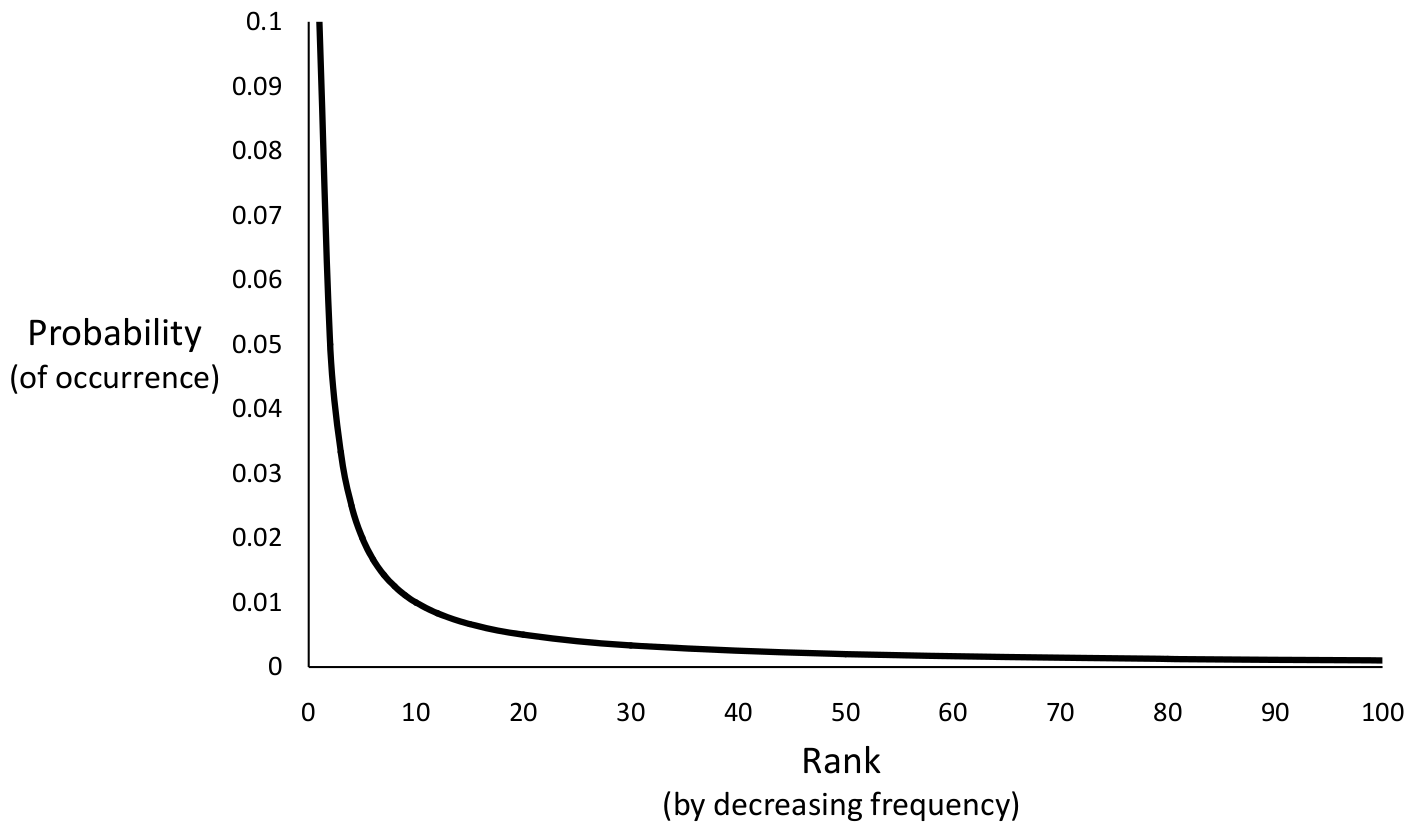
\includegraphics[width=0.7\textwidth]{zipf_law.png}
  \caption{Rank versus probability of occurrence for words assuming Zipf's law (rank $\cdot$ probability = 0.1)}
  \label{fig:ziplaw}
\end{figure}

This shows that a small number of words account for a very significant fraction of all text's size.

These terms make very poor index terms because of their low discriminative power. The job of a stopping component is to prevent them to appear in the index which size, in turn, results much smaller.

Depending on the retrieval model that is used as the basis of the ranking, removing these words usually has no impact on the search engine's effectiveness, and may even improve it.

However, the choice of words in \textit{stopwords list} may not be so easy: removing all common words makes impossible for the user to formulate queries like ``to be or not to be'', in which frequent words are put together to create meaningful content.

Some stoplists can be found at \url{https://github.com/igorbrigadir/stopwords}. They are taken from various sources such as Galago, Lucene, Terrier, NLTK and Gensim.

\subsubsection{Stemming}

The task of the stemming component (or stemmer) is to group words that are derived from a common stem (for instance, ``fish'' and ``fishing'') and replace them with that stem (``fish'').

Stemming generally produces improvements in ranking effectiveness because it increases the likelihood that words used in queries and documents will match.

There are two types of stemmers: rule-based and dictionary-based. A rule-based stemmer is a logic procedure that decide whether two words are related, usually based on knowledge of word suffixes, whereas a dictionary-based stemmer uses pre-created dictionaries of related terms to transform text.

The most popular rule-based stemmer to english is the Porter stemmer \footnote{\url{https://tartarus.org/martin/PorterStemmer}}.

An example of an hybrid approach (rule-based and dictionary-based) is the Krovetz stemmer \footnote{\url{https://sourceforge.net/p/lemur/wiki/KrovetzStemmer}}.

Another open source project called ``Snowball'' \footnote{\url{https://snowballstem.org}} was launched in 2001: it is a small string-handling language that can be used for several languages other than english.

Both stemming and stopwords removal do not follow a general rule and can be done aggressively, conservatively, or even be ignored - it all comes down to the type of text to process.

\subsubsection{Index creation}

Index terms are the parts of a document that are stored in the index and used in searching.

The simplest index term is a word, but not every word may be used for searching.

``Feature'' is a term often used in the field of machine learning to refer to a part of a text document that is used to represent its content, which also describes an index term.

All the indexed terms contribute to create the \textit{index vocabulary}.

The \textbf{index creation} component takes the output of the text transformation and creates the indexes or data structures that enable fast searching.

Inverted indexes are by far the most common form of index used by search engines. For each term indexed, an inverted index contains a list of documents called \textit{posting list}.

Elements of this list are called \textit{posting} and typically they are the documents in which the index term appears (see picture \ref{fig:inverted_index}).

Given the large number of documents in many search applications, index creation must be efficient, both in terms of time and space.

\begin{figure}
  \centering
  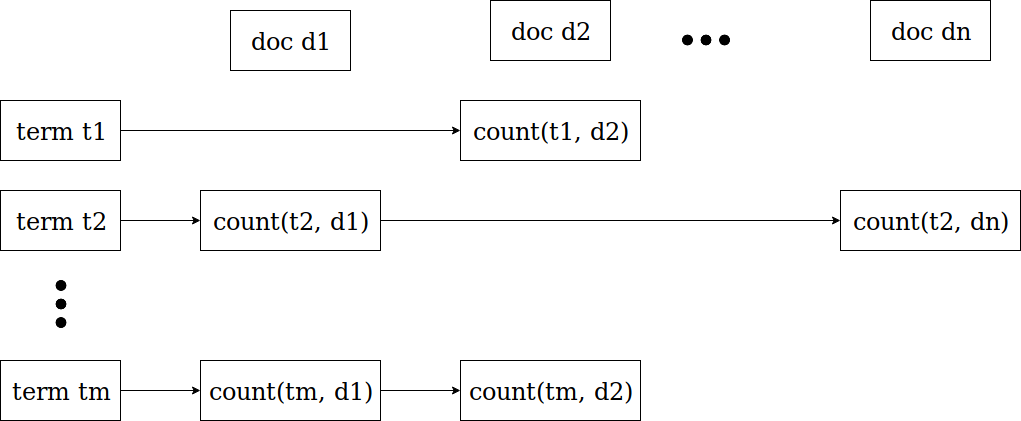
\includegraphics[width=0.9\textwidth]{inverted_index.png}
  \caption{An example of inverted index where postings are based on counting term occurrences in the document list}
  \label{fig:inverted_index}
\end{figure}

During index creation, other information may be collected such as \textbf{document statistics}, which may vary upon what is needed by the ranking model used by the search engine.

Generally, some useful information for traditional IR ranking models are the counts of index term occurrences (both words and more complex features) in individual documents, the positions in the documents where the index terms occurred, the lengths of documents in terms of the number of tokens and possibly many more.

Index term may also be associated to \textbf{weights} to reflect their relative importance in documents (see tf-idf model).

\subsection{Query process}

The major components of query process are user interaction, ranking, and evaluation (picture \ref{fig:query process}).

\begin{figure}
  \centering
  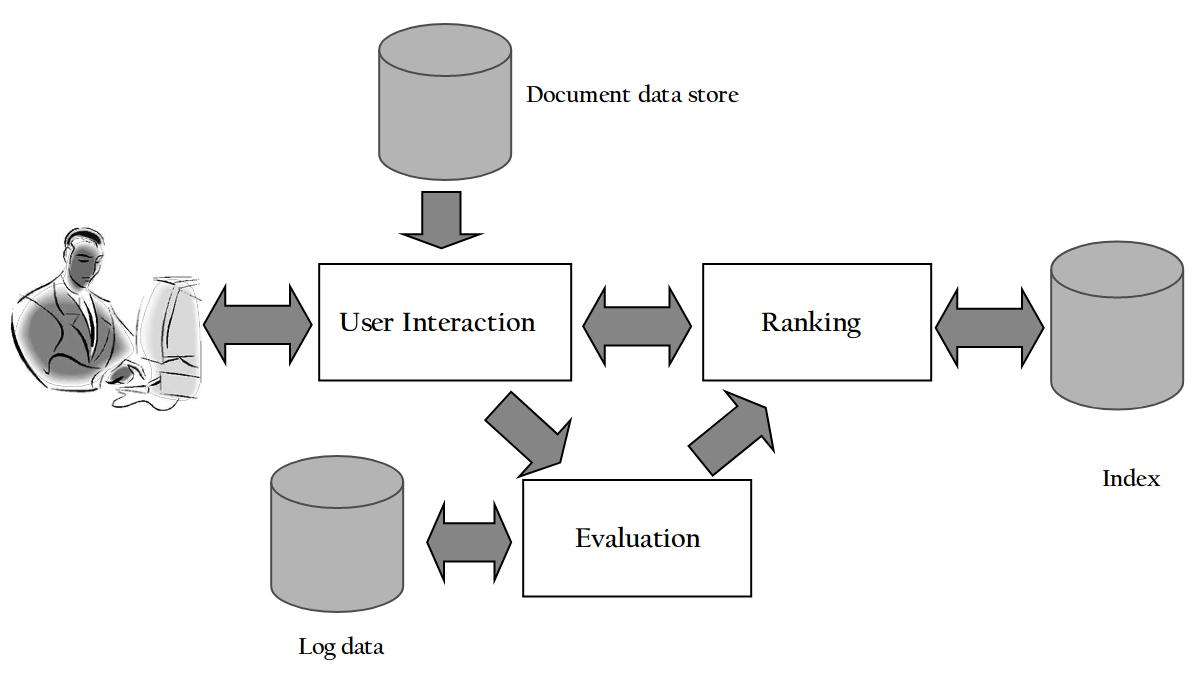
\includegraphics[width=0.9\textwidth]{query_process.png}
  \caption{The query process (picture taken from \cite{croftIR})}
  \label{fig:query process}
\end{figure}

The \textbf{user interaction} component provides the interface between the person doing the searching and the search engine.

Some tasks for this component include accepting the user's query and transforming it into index terms, display the ranked results and refining the query submitted.

The \textbf{ranking component} is the core of the search engine. It takes the transformed query from the user interaction component and generates a ranked list of documents using scores based on a retrieval model and the index created during the indexing process.

As happens with indexing, ranking have the desirable requirements of efficiency, which depends on indexes, and effectiveness, which depends on the retrieval model.

The \textbf{evaluation} is another important part of a search engine and, more generally, a fundamental concept in IR. Since the quality of a document ranking depends on how well it matches a user's expectations, it was necessary early on to develop evaluation measures and experimental procedures for evaluating retrieval systems and compare different ones.

\subsection{The ranking task}
\label{sssec:rnktsk}

Suppose that there are a set of queries $\mathcal{Q}=\{q_1, \dots q_M\}$ and a
set of documents $\mathcal{D} = \{d_1, \dots d_N\}$. Given a query $q \in  \mathcal{Q}$, and a document $d \in \mathcal{D}$, ranking is performed through a ranking function F(q, d):
$\mathcal{Q} \times \mathcal{D} \rightarrow \mathbb{R}$:

\begin{equation}
\label{eq:f}
\tag{Ranking model}
s_{q, d} = F(q, d)
\end{equation}

which gives a score $s_{q, d}$ for every pair (query $q$, document $d$) representing the relevance of $d$ w.r.t. $q$. Then, in order to obtain a ranking list $\pi$, elements in $\mathcal{D}$ are sorted by their score $s_{q, d}$.

\begin{equation}
\tag{Ranking list}
\pi = sort_{S_{q,d}}(\mathcal{D})
\end{equation}

\subsection{Retrieval}

In this section, two traditional probabilistic retrieval models are described and will be used later for comparison purposes against a neural retrieval model.

\subsubsection{Vector space model}

In this model, documents and queries are assumed to be part of a $t$-dimensional vector space, where $t$ is the number of index terms.

A document $D_i$ is represented by a vector $(d_{i1}, d_{i2}, \dots d_{in})$, where $d_{ij}$ represents the weight of the $j$th term.

A document collection containing $n$ documents can be represented as a matrix of term weights (see \ref{eq:tdmatrix}). 

Given this representation, documents can be ranked by computing the distance between the points representing the documents and the query.

In fact, in this model, it is implicitly assumed that relevance is related to the similarity of query and document vectors.

Several similarity measures can be used to compare terms. A common one is cosine similarity, that determines how similar two vectors $(\vec{v}, \vec{w})$ are:

\begin{equation}
\tag{Cosine similarity}
\label{eq:cosine}
\frac{\vec{v}^{\,t} \cdot \vec{w}}{\norm{\vec{v}}_2 \cdot \norm{\vec{w}}_2}
\end{equation}

where $\norm{\vec{v}}_2$ is the SRSS (euclidean norm - square root of the sum of squares).

The cosine correlation measures the cosine of the angle between the query and the document vectors.

A popular weighting scheme applied in the vector space model is \textit{tf-idf} \cite{croftIR}: tf stands for \textit{term frequency}, the frequency of index term occurrences in a document while idf stands for \textit{inverse document frequency}, the reciprocal of the frequency of index term occurrences over the entire collection of documents.

Idf weights are useful because they can give information about which terms are frequent or rare over the entire collection of documents.

If a term occurs in many times in the collection, then it cannot discriminate between documents and, consequently, is not useful for retrieval.

A typical formula for idf is $log \left( \frac{N}{n} \right)$ where $N$ is the number of documents indexed and $n$ is the number of documents that contain the term.

The effects of these two weights are combined by multiplying them (due to empirical results).

\subsubsection{Binary Independence model}

One early theoretical statement known as the \textbf{probability ranking principle} \cite{robertson}, encouraged the development of probabilistic retrieval models, which are the dominant paradigm today \cite{croftIR}.

The Probability Ranking Principle can be summed up as follow: ``if a retrieval system's response to each request is a ranking of the documents in the collection in order of decreasing probability of relevance, the effectiveness of the system will be the best that is obtainable on the basis of the data available''.

Given some assumptions, such as that the relevance of a document to a query ($p(R|d, q)$) is independent of other documents and it is binary (relevant / non relevant), it is possible to show that this statement is true.

A document is relevant if $p(R| d, q) > p(NR| d, q)$, i.e. if its probability of being relevant is greater than its probability of being non relevant.

Thanks to \ref{eq:bayes} the computation can unfold as follow:

\begin{equation}
    \label{eq:bayes}
    \tag{Bayes rule}
    P(R| d, q) = \frac{P(d, q | R) \cdot P(R)}{P(d, q)}
\end{equation}

\begin{equation}
    \label{eq:likelihood}
    P(d, q | R) \cdot P(R) > P(d, q | NR) \cdot P(NR) \implies \frac{P(d, q| R)}{P(d, q | NR)} > \frac{P(NR)}{P(R)}
\end{equation}

The left-hand side of equation \ref{eq:likelihood} is known as the \textbf{likelihood ratio}.

Thus, the highly ranked documents will be those that have a high likelihood of belonging to the relevant set.

To compute $P(d, q | R)$ and $P(d, q | NR)$ the following assumptions are made:

\begin{enumerate}
    \item documents are a combination of words, the relevant and non-relevant sets are probabilities distributions over word;
    \item each term is independent of one another (term independence, also known as the Naive Bayes assumption) and
    \item documents are represented as a vector of binary features, $D = (d_1, d_2, \dots d_t)$, where $d_i = 1$ if term i is present in the document, and 0 otherwise.
\end{enumerate}

So, $P(d, q | R)$ is the product of individual term probabilities ($p_i$ for a term $t_i \in d$) where $d$ is a relevant document while $P(d', q | NR)$ is the product of individual term probabilities ($s_i$ for a term $t_i \in d'$) where $d'$ is a non relevant document.

If there are no other information about the relevant set, then it can be assumed that $p_i$ is a constant and $s_i$ can be estimated by using the term occurrences in the whole collection as an approximation.

This shows that, in the absence of information about
the relevant documents, the term weight derived from the binary independence
model is very similar to an idf weight. There is no tf component, because the
documents were assumed to have binary features.

This model is generally known as the \textbf{binary independence model} (BIM).

The absence of a tf component makes a significant difference to the effectiveness of the ranking, and most
effectiveness measures will drop by about 50\% if the ranking ignores this information.

It turns out, however, that the BIM is the basis for one of the most effective and popular ranking algorithms, known as \textbf{BM25}.

BM25 extends BIM scoring function to include document and query term weights.

The extension is based on probabilistic arguments and experimental validation, but it is not a formal model.

\subsubsection{Probabilistic language modelling}

The simplest form of language model, known as unigram language model, is a probability distribution over the words in the language. This means that the language model associates a probability of occurrence with every word in the index vocabulary for a collection.

An n-gram model predicts a word based on the previous n - 1 words. The most common n-gram models are bigram and trigram models.

In a language modelling based approach, documents are ranked by the posterior probability $P (d|q)$ that a document $d$ is relevant w.r.t. a query $q$.

In a \textbf{query likelihood retrieval model} documents are ranked by the probability that the query text could be generated by the document language model.

This is a model of topical relevance, in the sense that the probability of query generation is the measure of how likely it is that a document is about the same topic as the query.

An obvious estimate of such distributions is just the frequency of a term in the query over a document.

The major problem with this estimate is that if any of the query $q$ words are missing from a document $d$, the score given by the query likelihood model for $p (d|q)$ will be zero. This is clearly not appropriate for long queries.

\textbf{Smoothing} is a technique for avoiding this estimation problem and overcoming data sparsity.

The general approach to smoothing is to lower the probability estimates for words that are seen by multiplying them by a certain quantity $1- \alpha$ in the document text, and give the probability left over $\alpha$ to the estimates for the words that are not seen in the text.

The estimates for unseen words are usually based on the frequency of occurrence of words in the whole document collection. \\

Both tf-idf and language modelling based approaches estimate document relevance based on the count of only the query terms in the document; the position of these occurrences and the relationship with other terms in the document are ignored.

\section{Experimental evaluation}

As previously introduced, evaluation is a core issue in IR. It is an expensive activity both in terms of time and energies needed to perform it, in fact early experiments conducted by Cleverdon took years to be concluded (the first, Cranfield-I, ran from 1957 to 1961 and the second, Cranfield-II, ran from 1963 to 1966).

\subsection{The Cranfield paradigm}

The first person to set the stage for IR experimental evaluation was Cyril Cleverdon, who developed the Cranfield paradigm (\cite{harmaneval}).

After WW2, there has been a huge increase in the volume of scientific papers and so, an efficient way to index and retrieve them was required, based on the information needs of researchers.

\subsubsection{Cranfield-I}

Back in 1955 the first experiment (called \textit{Cranfield-I}) began: 18000 papers and reports from the field of aerodynamics were manually indexed on the basis of 4 different indexing systems.

It took 2 years of work before the indexing was completed. After that, Cleverdon asked the authors of the indexed documents to select some of them and frame a question that could be answered by that document (thus, avoiding the need of explicit relevance judgements).

The searching phase of the experiment required using each of the 4 indexes to manually search for the documents, recording the search time and the success (or failure) of the search.

The search failed an average of 35\% of the time, with no significant differences among the indexing systems.

Cleverdon was able to discover the real problem simply because of the huge amount of data that was examined in the failure analysis.

The issue was not the specific indexing system used, but rather the actual content descriptors that were used to index each document.

\subsubsection{Cranfield-II}

The problem of how to select content descriptors for indexing, and an increasing interest in evaluation issues, led Cleverdon to continue his investigations in a second experiment (called \textit{Cranfield-II}).

That time, the experiment was conducted with 1200 documents and 300 questions. Cleverdon thought that it was critical to first build the test collection (documents, questions, and relevance judgments), and then do the experiments on the indexing and searching.

The documents needed to be ones that researchers would naturally be search, the questions needed to reflect ones they might ask and the relevance judgments needed to mirror the type of judgments they would make for documents they examined in the search process.

The papers along with their references were sent to their authors who were asked to formulate the basic problem in the form of a search question, and then assess the relevance of each paper w.r.t. that question.

There were 173 useful forms returned, with an average of 3.5 questions per form. The document collection was built by merging the 173 source documents with their cited documents (those that had been previously sent to the authors for judgments), and 209 additional similar documents, for a total of 1400 documents.

Five graduate students spent the summer of 1963 making preliminary (and liberal) judgments for these 361 questions against all 1400 documents.

The goal of Cranfield 2 was to examine in more depth the various properties of index methodologies.

\begin{table}[H]
\centering
\begin{tabular}{ c  c  c | c }
& \textbf{Relevant} & \textbf{Non-Relevant} & \\
\hline
\textbf{Retrieved} & a & b & a + b \\
\textbf{Not retrieved} & c & d & c + d \\ \hline
& a + c & b + d & \\
\hline
\end{tabular}
\caption{Categories of document in searching}
\label{tab:measures}
\end{table}

The metrics used referred to the well-known categories shown in table \ref{tab:measures}; at that time they were called \textbf{``Recall Ratio''} defined as $\frac{a}{a + c}$, and the \textbf{``Precision Ratio''} defined as $\frac{a}{a + b}$. Cleverdon liked both the simplicity of recall and precision and the fact that they directly described a user's experience.

An important outcome of these experiments was the Cranfield paradigm for evaluation.

Today, for evaluation purposes, it is common the use of a static test collection of documents, questions, and relevance judgments, often with standard recall and precision metrics.

The collection of scientific documents, the selection of users that would heavily use this collection, and the careful definition of relevance based on how these particular users might judge documents were critical pieces of the Cranfield paradigm.

Other important components of the experiment were the careful modeling of the task being tested and the strict separation of the building of the test collection from the experimentation itself.

\subsection{International IR evaluation campaigns}

Nowadays there are public, large-scale evaluation campaigns at international level that produce large experimental collections and compare state-of-the-art systems and algorithms \cite{croftIR}.

Relevant and long-lived examples are the Text REtrieval Conference (TREC) \cite{TREC} in the United States, the Conference and Labs of Evaluation Forum (CLEF) initiative in Europe, and the NII Testbeds and Community for Information access Research (NTCIR) in Japan and Asia.

In this context, it is worth to mention some important conferences in IR such as SIGIR \footnote{acronym for Special Interest Group on Information Retrieval}, considered the most important in the field of IR (internationally) and ECIR \footnote{European Conference on Information Retrieval} (in Europe).

\subsubsection{TREC}

TREC (co-sponsored by the National Institute of Standards and Technology (NIST) and U.S. Department of Defense) was started in 1992 as part of the TIPSTER Text program.

Its purpose is to support research within the IR community by providing the infrastructure necessary for large-scale evaluation of text retrieval methodologies.

In particular, the TREC workshop series has the following goals:

\begin{itemize}
 \item to encourage research in IR based on large test collections;
 \item to increase communication among industry, academia, and government by
creating an open forum for the exchange of research ideas;
 \item to speed the transfer of technology from research labs into commercial
products;
 \item to increase the availability of appropriate evaluation techniques for
use by industry and academia.
\end{itemize}

For each TREC, NIST provides a test set of documents and questions.

Participants run their own retrieval systems on the data, and return to NIST a
list of the retrieved top-ranked documents. NIST pools the individual results,
judges the retrieved documents for correctness, and evaluates the results.

The TREC cycle ends with a workshop that is a forum for participants to share
their experiences.

As already stated, relevance is a complex concept. TREC uses the following definition:

\begin{quote}
\textbf{Working definition of relevance}: if was to write a report on the subject of the topic and would use the information contained in the document in the report, then the document is relevant.
\end{quote}

Only binary judgments (relevant or not relevant) are made, and a document
is judged relevant if any piece, however small, of it is relevant. This follows the \textbf{scope
hypothesis} which states that relevance matching could happen in any part of a document, as opposed to the \textbf{verbosity hypothesis} where the whole document is required to be
relevant to a query (global relevance).

Judging is done using a \textbf{pooling technique} on the set of documents used for the task that year: only a subset of documents returned by different retrieval systems are manually judged.

\subsection{Formal framework}

In this section I will present a detailed explanation of experimental evaluation and the metrics typically applied to measure the performance of an IR search engine, based on the formalization given in \cite{virtue}.

A test collections is a triple: $(\mathcal{D}, \mathcal{T}, \mathcal{GT})$, where $\mathcal{D}$ is a set of documents, also called collection of documents, $\mathcal{T}$ is a set of topics, which express user information needs and $\mathcal{GT}$ is the ground truth, defined below.

Let REL be a set of relevance degrees and let $\succ$ be a total order relation on REL so that $(REL, \succ)$ is a total ordered set. $min(REL)$ is what defines a non-relevant degree.

The ground truth can be formalized in the following way:

\begin{definition}{\textbf{Ground truth}}

The ground truth is a function:
\begin{align*}
  \mathcal{GT} \colon \mathcal{T} \times \mathcal{D} &\to REL\\
  (t, d) &\mapsto rel.
\end{align*}

\end{definition}

The recall base is linked to the definition of ground truth and it is the total number of relevant documents for a given topic t:

\begin{definition}{\textbf{Recall base}}

The recall base is a function:
\begin{align*}
  \mathcal{RB} \colon \mathcal{T} &\to \mathbb{N}\\
  t &\mapsto \mathcal{RB}_t = |\{ d \in \mathcal{D} | \mathcal{GT}(t, d) \succ min(REL) \}|.
\end{align*}
\end{definition}

An experiment in IR, also called \textbf{run}, is the output of an IR system which usually is composed by a set of ranked lists of documents – one for each topic.

\begin{definition}{\textbf{Run}}

A run is a function:
\begin{align*}
  \mathcal{R} \times \mathcal{T} &\to \mathcal{D}^n\\
  t &\mapsto r_t = (d_1, d_2, \dots d_n).
\end{align*}
where $r_t$ documents $d_1, d_2, \dots d_n$ are all different.

\end{definition}

\subsubsection{Metrics}
\label{ssec:metrics}

The most used metrics in IR are based on a rank-based comparisons of the
retrieved result set $\mathcal{R}$ ($\mathcal{R}_q$ is a run w.r.t. a query q) to an ideal ranking of documents $\mathcal{I}$, determined by manual judgments or implicit feedback from user behavior data (ground truth).

These metrics are typically computed at a rank position (k) and then
averaged over all queries in the test set.

Before presenting them, a useful definition is the \textbf{relevance score} of a run:

\begin{definition}{\textbf{Relevance score}}

Given a run $\mathcal{R}(t) = r_t$, its relevance score is a function:
\begin{align*}
  \mathcal{\hat{R}} \colon \mathcal{T} \times \mathcal{D}^n &\to REL^n\\
  (t, r_t) &\mapsto \hat{r_t} = (rel_1, rel_2, \dots rel_n).
\end{align*}
where $\hat{r_t}[j] = \mathcal{GT}(t, r_t[j])$
\end{definition}

For simplicity, from now on, I assume that REL is simply a binary set (\{rel, non rel \}) which can be weighted as $\{0, 1\}$, so $\hat{r_t}$ is a binary vector. \\

In the following, formal definitions of the metrics used in Cranfield experiment (precision and recall) are given.

Precision indicates the ratio of relevant documents retrieved by a system over the total number of retrieved documents:

\begin{definition}{\textbf{Precision}}\\

Let $\mathcal{R}(t)=r_t$ be a run with length $N \in \mathbb{N}^+$ where $t \in \mathcal{T}$ is a given topic. Precision is defined as follow:
\begin{align*}
P_{r_t} = \frac{1}{N} \sum_{j = 1}^N \hat{r_t}[j]
\end{align*}

\end{definition}

It's worth notice that precision differs from \textbf{accuracy} (the rate of correct predictions), often used for classification task in machine learning. In fact, the task considered here is document ranking which is different from document classification.\\

Recall indicates the ratio of relevant documents retrieved by a system over the total number of relevant documents for a given topic (i.e. its recall base):

\begin{definition}{\textbf{Recall}}\\

Let $\mathcal{R}(t)=r_t$ be a run with length $N \in \mathbb{N}^+$ where $t \in \mathcal{T}$ is a given topic. Recall is defined as follow:
\begin{align*}
R_{r_t} = \frac{1}{\mathcal{RB}_t} \sum_{j = 1}^N \hat{r_t}[j]
\end{align*}

\end{definition}

By looking at the context, one measure may be more important than the other
(e.g. in web search it is more important to get a high precision on the first
page than a high recall considering all pages retrieved).

These two quantities trade off against one another: it is possible to get a high recall
but very low precision by retrieving all documents for all queries, in fact
recall increases as the number of documents retrieved increase.

Precision and recall can be defined at different levels of cut-off: this means that a run is partially evaluated up to a certain threshold / cutoff k. The notation used may vary, for instance to indicate precision at k one may use either $P@k$ or $P[k]$.

Average precision is a measure that combines precision and recall.

It is \textbf{top-heavy}: it means that it assign more weight to a relevant document placed at high rank than a relevant document placed at low rank.

\begin{definition}{\textbf{Average Precision}}\\

Let $\mathcal{R}(t)=r_t$ be a run with length $N \in \mathbb{N}^+$, where $t \in \mathcal{T}$ is a given topic and $RB_t$ its recall base. Average Precision is defined as follow:
\begin{align*}
AP_{r_t} = \frac{1}{RB_t} \sum_{j = 1}^N \hat{r_t}[j] \cdot \frac{\sum_{h = 1}^j \hat{r_t}[h]}{j}
\end{align*}

\end{definition}

The MAP value for a test collection is the arithmetic mean of average precision values for each topic.

\begin{definition}{\textbf{Mean Average Precision}}\\

Let $\mathcal{S}$ by an IR search engine, $\mathcal{T}$ a set of topics and $r_t$ the run generated by $\mathcal{S}$ associated to the topic $t \forall t \in \mathcal{T}$. Mean Average Precision is defined as follow:

\begin{align*}
MAP_{\mathcal{T}} = \frac{\sum_{t \in \mathcal{T}} AP_{r_t}}{|\mathcal{T}|}
\end{align*}

\end{definition}

This metric has the drawback of weighing each topic equally in the final reported number, even if many documents are relevant to some queries whereas very few are relevant to other queries - as happens with the results reported in experimental section (\ref{sec:comparison}).


Precision, Recall, Average Precision and MAP can only handle binary judgments (relevant/not relevant),
whereas  cumulative gain family of measures in IR can handle graded relevance degrees.

The premise of these measures is that highly relevant documents appearing lower in a search result list should be penalized.

\begin{definition}{\textbf{Cumulative gain (CG)}}\\

Let $\mathcal{R}(t)=r_t$ be a run with length $N \in \mathbb{N}^+$, where $t \in \mathcal{T}$ is a given topic, $\mathcal{RB}_t$ its recall base and $1 \leq j \leq N$ the cutoff up to which the run should be evaluated. $CG[j]$ is defined as follow:

\begin{align*}
CG[j] = cg_{r_t} = \sum_{k = 1}^j \hat{r_t}[k]
\end{align*}

\end{definition}

The normalized version of CG (nCG) definition uses the concept of ``ideal run'' which is a run that, given a topic $t \in \mathcal{T}$, has retrieved all relevant documents and place them in the best possible order. Formally:

\begin{definition}{\textbf{Ideal run I(t)}}\\

Given a topic $t \in \mathcal{T}$, the ideal run $\mathcal{I}(t)=i_t$ is a run which satisfies the following constraints:

\begin{enumerate}
    \item recall base: $\forall t \in \mathcal{T}, |\{ 1 \leq i \leq N \quad \mathcal{GT}(t, i_t[j]) \succ min(REL) \}| = RB_t$
    \item ordering: $\forall t \in \mathcal{T} \quad \forall j,k \quad j < k \implies i_t[j] \succeq i_t[k]$
\end{enumerate}

\end{definition}

\begin{definition}{\textbf{Normalized cumulative gain (nCG)}}\\

nCG at position j is defined as the ratio between the CG of the considered run $R(t)=r_t$ and the CG of the ideal run $\mathcal{I}(t)=i_t$:

\begin{align*}
nCG[j] = \frac{cg_{r_t}[j]}{cg_{i_t}[j]}
\end{align*}

\end{definition}

The discounted cumulative versions of these metrics give another view of the run by weighting down the gain received through documents found later in the ranked results, thus giving more
importance to the early positions in ranking. Both discounted cumulative gain (DCG) and normalized DCG (nDCG) are top-heavy.

DCG and nDCG uses the following definition of discounted gain (dg):

\begin{definition}{\textbf{Discounted gain (dg)}}

Let $\mathcal{R}(t) = r_t$ be a run with length $N \in \mathbb{N}^+$, where $t \in \mathcal{T}$ is a given topic and a log base $b \in \mathbb{N}^+$; for all $1 \leq k \leq N$, the discounted gain is defined as follow:

\begin{align*}
dg_{r_t}^b = \begin{cases}
\hat{r_t}[k] & \text{if k < b}\\
\frac {\hat{r_t}[k]}{log_b k} &\text{otherwise}
\end{cases}
\end{align*}

\end{definition}

So, DCG can be defined as follow:

\begin{definition}{\textbf{Discounted cumulative gain (DCG)}}\\

Let $\mathcal{R}(t) = r_t$ be a run with length $N \in \mathbb{N}^+$, where $t \in \mathcal{T}$ is a given topic and a log base $b \in \mathbb{N}^+$.
The discounted gain at some cutoff j is:

\begin{align*}
DCG[j]_{r_t}^b = \sum_{k=1}^j dg_{r_t}^b [k]
\end{align*}

\end{definition}

The respective normalized version uses the ideal run, just like nCG:

\begin{definition}{\textbf{Normalized discounted cumulative gain (nDCG)}}\\

nDCG at position j is defined as the ratio between the DCG of the considered run $R(t)=r_t$ and the DCG of the ideal run $\mathcal{I}(t)=i_t$:

\begin{align*}
nCG[j] = \frac{DCG[j]_{r_t}^b}{DCG[j]_{i_t}^b}
\end{align*}

\end{definition}

\section{Advanced topics in IR}

Recently, different approaches to IR have been explored by researchers.

Here, two new areas are presented: one, called \textbf{learning to rank} (LTR) emerged from the intersection of machine learning, IR and natural language, and the other, called \textbf{Neural IR}, focuses on the application of neural network to IR tasks.

Unlike classical LTR models and non-neural approaches to IR, Neural IR techniques are data-hungry, requiring large scale training data before they can be deployed.

Those two areas are not strictly separated: in fact neural networks have been employed over the years as LTR models. However, Neural IR exploits more in depth neural networks and can use them even without the need of labelled data (i.e. ground truth).

\subsection{Learning to Rank}

Learning to rank refers to machine learning techniques applied in a ranking task.

Liu in \cite{learntorank} give the following general definition:

\begin{quote}
``(\dots) LTR is the task to automatically construct a ranking model using
training data, such that the model can sort new objects according to their
degrees of relevance (...)''
\end{quote}

LTR models take as input a numerical vector $ \vec{x} \in \mathbb{R}^n$ which represents a rankable item (e.g. a document) given some context (e.g.
a user-issued query).

The ranking model $F: \vec{x} \rightarrow \mathbb{R}^n$ is then trained to map the
vector to a real-valued score such that relevant items are scored higher.

\subsubsection{Training and testing}

Let $\mathcal{Q}=\{q_1, \dots q_M\}$ and $\mathcal{D} = \{d_1, \dots d_N\}$ be
the queries and documents set respectively.

Suppose that $\mathcal{Y} = \{1, \dots l\}$ is a set of grades for which exists
a total order $l \succ l-1 \succ \dots \succ 1$.

Let S be the training set: $S=\{(q_i,d_j), y_{i,j}\}, 0 \leq i \leq m,
0 \leq j \leq n$ where each pair (query $q_i$, document $d_i$) is associated to a relevance score $y_{i,j}$.

The aim is to train a model $F(q,d)$ based on the training set $S$, that can assign
a score to any pair $(q,d)$.

\begin{figure}[H]
  \centering
  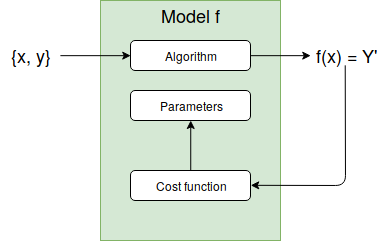
\includegraphics[width=0.7\textwidth]{model_ltr.png}
  \caption{Learning to rank abstract model}
  \label{fig:model_ltr}
\end{figure}

Ranking uses the output of $F$ to sort documents in $\mathcal{D}$ by the scores obtained.

\subsubsection{Learning to rank approaches}

Liu in \cite{learntorank} categorizes 3 different LTR approaches on the basis of training objectives (i.e. loss function, explained in next chapter):

\begin{itemize}
 \item \textbf{Pointwise approach}: Typically, a regression or classification
model is trained to predict a relevance label $y_{q,d}$ given $\vec{x}_{q,d}$. During training each document is considered separately;
 \item \textbf{Pairwise approach}: Binary classification model trained to
predict which document in a given pair is the most relevant with respect to
a certain query.
Pairwise loss minimizes the average number of inversions in ranking
(i.e. $y_{i,h} \succ y_{i_k}$ but document $d_k$ is ranked higher than
$d_h$ w.r.t. query $q_i$). This approach is sensible to noise as a mis-labeled document
can results in a huge number of mislabeled pairs.
 \item \textbf{Listwise approach} This approach considers the entire list of
documents and try to come up with an ordering that optimizes an IR
measure (i.e. nDCG). The resulting optimization problem is more challenging
than those in the pointwise or pairwise approach, due to the non-continuous
and non-differentiable loss function.
\end{itemize}

The pointwise and pairwise approaches transform the ranking problem into
classification, regression, and ordinal classification problem.
The listwise approach addresses the learning-to-rank problem in the most natural
way, by taking document lists as instances in the learning process.

The main differences among the approaches actually lies in the loss functions
employed.

Similarly to LTR, in Neural IR the ranking objective function adopted can be
categorized in the three categories mentioned in the list above.

\subsection{Neural IR}

Since the turn of the decade, there have been dramatic improvements in performance in computer vision, speech recognition, and machine translation task. These breakthroughs were largely fuelled by recent advances in neural network models, which have captured the attention of IR community.

Compared to traditional LTR models that employ machine learning techniques over hand-crafted IR features (i.e. features manually computed from input text which are not learned), neural models can learn representations of language from raw text.

Such representations can bridge the gap between query and document vocabulary and directly address the \textbf{vocabulary mismatch problem} (when different words are used to express the same concept) - which often occurs when comparing pairs of short-texts.

This turns out to be particularly useful, for instance, in search task where there is a lexical gap between search queries and retrieved documents (e.g. in bug and feature location, where queries are expressed in natural language and documents are expressed in code / some programming language).

Many Neural IR models depend on learning good
low-dimensional vector representations - or \textbf{embeddings} - of query and document text, and using them within traditional IR models or in conjunction with simple similarity metrics (e.g., cosine similarity).

Unlike classical IR models, these new machine learning based approaches are data-hungry and require large scale training data before they can be deployed.

Motivations for Neural IR include increased availability of big data, more powerful computing resources, and better neural network models and parameter estimation techniques \cite{neurev}.

IR community interest for neural approaches begun when Mikolov and Dean et al. \cite{w2v} proposed \textbf{Word2Vec}, a model and estimation procedure for word embeddings (also known as distributed term representations).

The availability of Word2Vec code and existing pre-trained embeddings has provided one of the key avenues for early work on Neural IR, especially for extending traditional IR models.

\section{Resources}

There are several open source resources for IR, some of which are used in this work. Among them, the most known are the search engines Terrier (\cite{terrier}), Lucene and Galago and the evaluation tool trec eval.

\subsection{Terrier}

Terrier IR Platform is a modular open source software written in Java for the rapid development of large-scale IR applications. Terrier was developed by members of the IR Research Group, Department of Computing Science, at the University of Glasgow.

A core version of Terrier is available as open source software under the Mozilla Public License (MPL), with the aim to facilitate experimentation and research in the wider IR community.

\subsection{Trec eval}

Trec eval is the standard tool used by the TREC community for evaluating an ad hoc retrieval run, given the results file and a standard set of judged results. 

It contains several implementations of the most common metrics cited in the evaluation section.

Other open-source toolkits have also been made available to enable and ease repeatable IR search experiments: Galago, Lemur and Lucene \cite{croftIR}.
